\documentclass[12pt]{iopart}

% packages
\usepackage{graphicx}
\usepackage{IEEEtrantools}
\usepackage{amsmath}

% Custom macros
\gdef\mcm{r@{.}l@{ ± }r@{.}l} % Multi Column Measurement; Used for decimal aligning & ± aligning
\gdef\mch#1{\multicolumn{4}{l}{#1}} % Multi Column Header; Used for decimal aligning & ± aligning
\gdef\mcmnd{r@{ ± }l} % Multi Column Measurement No Decimal; Used for ± aligning when the values don't need a decimal point
\gdef\mchnd#1{\multicolumn{2}{l}{#1}} % Multi Column Header No Decimal; Used for  ± aligning when the values don't need a decimal point
\gdef\sci#1#2{#1 \times 10^{#2}}
\gdef\units#1{~\mathrm{#1}}
\graphicspath{{./images/}}

%%%%%%%%%%%%%%%%%%%% Document Starts %%%%%%%%%%%%%%%%%%%%
\begin{document}

%%%%%%%%%%%%%%%%%%%% Title Page %%%%%%%%%%%%%%%%%%%%
\title{DTMF Signaling}
\author{Ali Mortada, Xavier Valencia, James Phommachanh}
\vspace{10pt}
\begin{indented}
  \item[]Mt.~San Antonio College, ENGR 285, CRN 43464
  \item[]June 14, 2024
\end{indented}
\newpage

%%%%%%%%%%%%%%%%%%%% Objective 1 %%%%%%%%%%%%%%%%%%%%
\section{Objective 1: Encoding Program}

This is the section for the first objective. \newline

What to talk about:
\begin{itemize}
    \item What \verb|createPureToneData| does
    \item What \verb|toneList| is
    \item What the for loop does
\end{itemize}


% figures look like this and go into the images folder
%\begin{figure}[h!tbp]
%  \begin{center}
% \item[]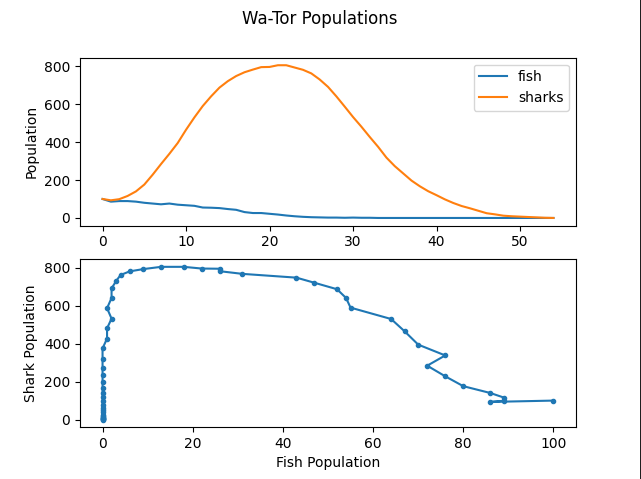
\includegraphics[width=0.6\textwidth]{figure1.png}
%  \caption{\label{fig:figure1}
%  Horizontal motion vs. time. 
%  It is clear that the horizontal motion increases as its step is increased by 3.
%  }
%  \end{center}
%\end{figure}

\pagebreak

%%%%%%%%%%%%%%%%%%%% Objective 2 %%%%%%%%%%%%%%%%%%%%
\section{Objective 2: Slicing Data}

This is the section for the second objective. \newline

What to talk about:
\begin{itemize}
    \item Function has to divide the data into equally sized parts which depends on the number of inputs
    \item Iterates through the save data with a step size of the slice size
    \begin{itemize}
        \item Uses another nested for loop that only adds signals that are not pauses (signal is not equal to 0)
        \item If a signal is found, it is added to the data list that the function returns
    \end{itemize}
\end{itemize}

\pagebreak


%%%%%%%%%%%%%%%%%%%% Objective 3 %%%%%%%%%%%%%%%%%%%%
\section{Objective 3: Calculating Approximate Fourier Coefficients}

This is the section for the third objective. \newline

What to talk about:
\begin{itemize}
    \item T is the length of the slice we are analyzing
    \item Integral is just a sum, so we can approximate it by multiplying each data point in the slice with its respective trig function
    \begin{itemize}
        \item $t$ is the data point divided by the frame rate
    \end{itemize}
    \item Coefficient returned is the Euclidean norm of $a$ and $b$
\end{itemize}

\pagebreak

%%%%%%%%%%%%%%%%%%%% Objective 4 %%%%%%%%%%%%%%%%%%%%
\section{Objective 4: Outputting Decoded Digits}

This is the section for the fourth objective. \newline

What to talk about:
\begin{itemize}
    \item Iterate through each data point in the sliced data
    \begin{itemize}
        \item Create a list of low coefficients using the \verb|calculate_coefficient| function and passing in the data point and each low frequency
        \item Repeat for the high coefficients
    \end{itemize}
    \item Find the low frequency from the index of the first appearance of the maximum low coefficients value
    \item Repeat for the high frequency
    \item Pass in the previously found low and high frequencies into \verb|decode_freqs|, and if it is not -1, append it to the list of stored numbers
\end{itemize}

\pagebreak

%%%%%%%%%%%%%%%%%%%% Extension %%%%%%%%%%%%%%%%%%%%
\section{Extension: Handling Alphabetical Messages}

For the extension, we decided to implement handling alphanumeric messages (apparently we don't know how to read instructions properly).
To do this, we had to extend the list of low and high frequencies, since the original four low frequencies and three high frequencies cannot make thirty-six unique combinations.
Thus, we added two new frequencies to the low frequencies list, $1037 \units{Hz}$ and $1144 \units{Hz}$, and three new frequencies to the high frequencies list, $1633 \units{Hz}$, $1776 \units{Hz}$, and $1919 \units{Hz}$.
These frequencies were chosen arbitrarily by our good friend Chad, and Figure \ref{fig:extended_freq_table} shows the mapping of each alphanumeric symbol to its pair of low and high frequencies. 
In the \verb|DTMFwrite| program, the arrays for each frequency were replaced by a frequency map matching each symbol to its pair of frequencies, and this map was used to populate \verb|toneList|.

\begin{figure}[h!tbp]
  \begin{center}
 \item[]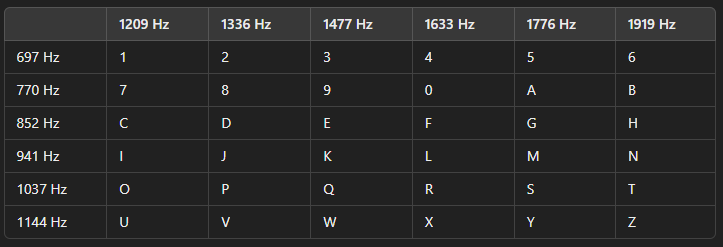
\includegraphics[width=0.8\textwidth]{extended_freq_table.png}
  \caption{\label{fig:extended_freq_table}
  Extended frequency table matching each alphanumeric symbol to a pair of low and high frequencies.
  }
  \end{center}
\end{figure}

The \verb|slice_data()| function was also slightly modified to handle more symbols.
The variable \verb|slice_size| was redefined to be smaller to ensure a more accurate tone was recorded.
New variables \verb|overlap| and \verb|sound_cutoff| were also defined to make sure the full tone was recorded and to filter out signals with no sound, respectively.
The for loop now checked to see if the current signal was above the cutoff threshold before adding it to the data list -- otherwise, it would skip over the overlap.

The code was now theoretically ready to handle alphanumeric messages.
However, when it was tested, we found that the program would output multiple copies of the same symbol for each symbol in the message, as shown in Figure \ref{fig:extension_output_bad}.
To fix this, code was added to check if the current character is equal to the previously stored character -- if it is not, then it is added to the list of stored characters.
This seemed to fix the issue, but it added the limitation of being unable to read messages that have two or more of the same symbol consecutively, only outputting one copy of the letter.
A sample output after the fix can be seen in Figure \ref{fig:extension_output}.

\begin{figure}[h!tbp]
  \begin{center}
 \item[]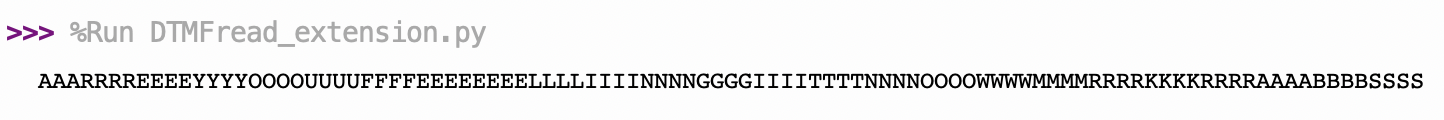
\includegraphics[width=1\textwidth]{extension_output_bad.png}
  \caption{\label{fig:extension_output_bad}
  Initial output with test message "AREYOUFEELINGITNOWMRKRABS". 
  Notice how each letter has 3-4 multiples in the output.
  }
  \end{center}
\end{figure}

\begin{figure}[h!tbp]
  \begin{center}
 \item[]
\includegraphics[width=0.6\textwidth]{extension_output.png}
  \caption{\label{fig:extension_output}
  Initial output with test message "AREYOUFEELINGITNOWMRKRABS" after fixing repeated symbol issue. Notice how the double E in "FEELING" only has one E outputted.
  }
  \end{center}
\end{figure}

It is worthy to note that after implementing this extension, it takes noticeably longer for both the \verb|DTMFread| and \verb|DTMFwrite| programs to execute.
This is likely because it has to map each symbol to its frequency pair instead of just reading from an array for each frequency.
Both programs also contain multiple nested loops, so it is not unreasonable to assume that the time complexity of each program increases quadratically with an increasing number of symbols.


\end{document}
%%%%%%%%%%%%%%%%%%%% Document Ends %%%%%%%%%%%%%%%%%%%%